\section{Implementation}\label{sec:implementation}
While M1 GPUs don't support double precision, 
they are a promising target for scientific computing \cite{Kenyon2022}.

Our implementation utilizes \textit{SymPy} to derive expressions for each $\Omega(f_i)$ over the free variables $\rho, u, f$ from equation \ref{eqn:cm-mrt}. These expressions are eventually templated into WGSL compute shaders, see Fig \ref{fig:architecture}.

\begin{figure*}
\begin{center}
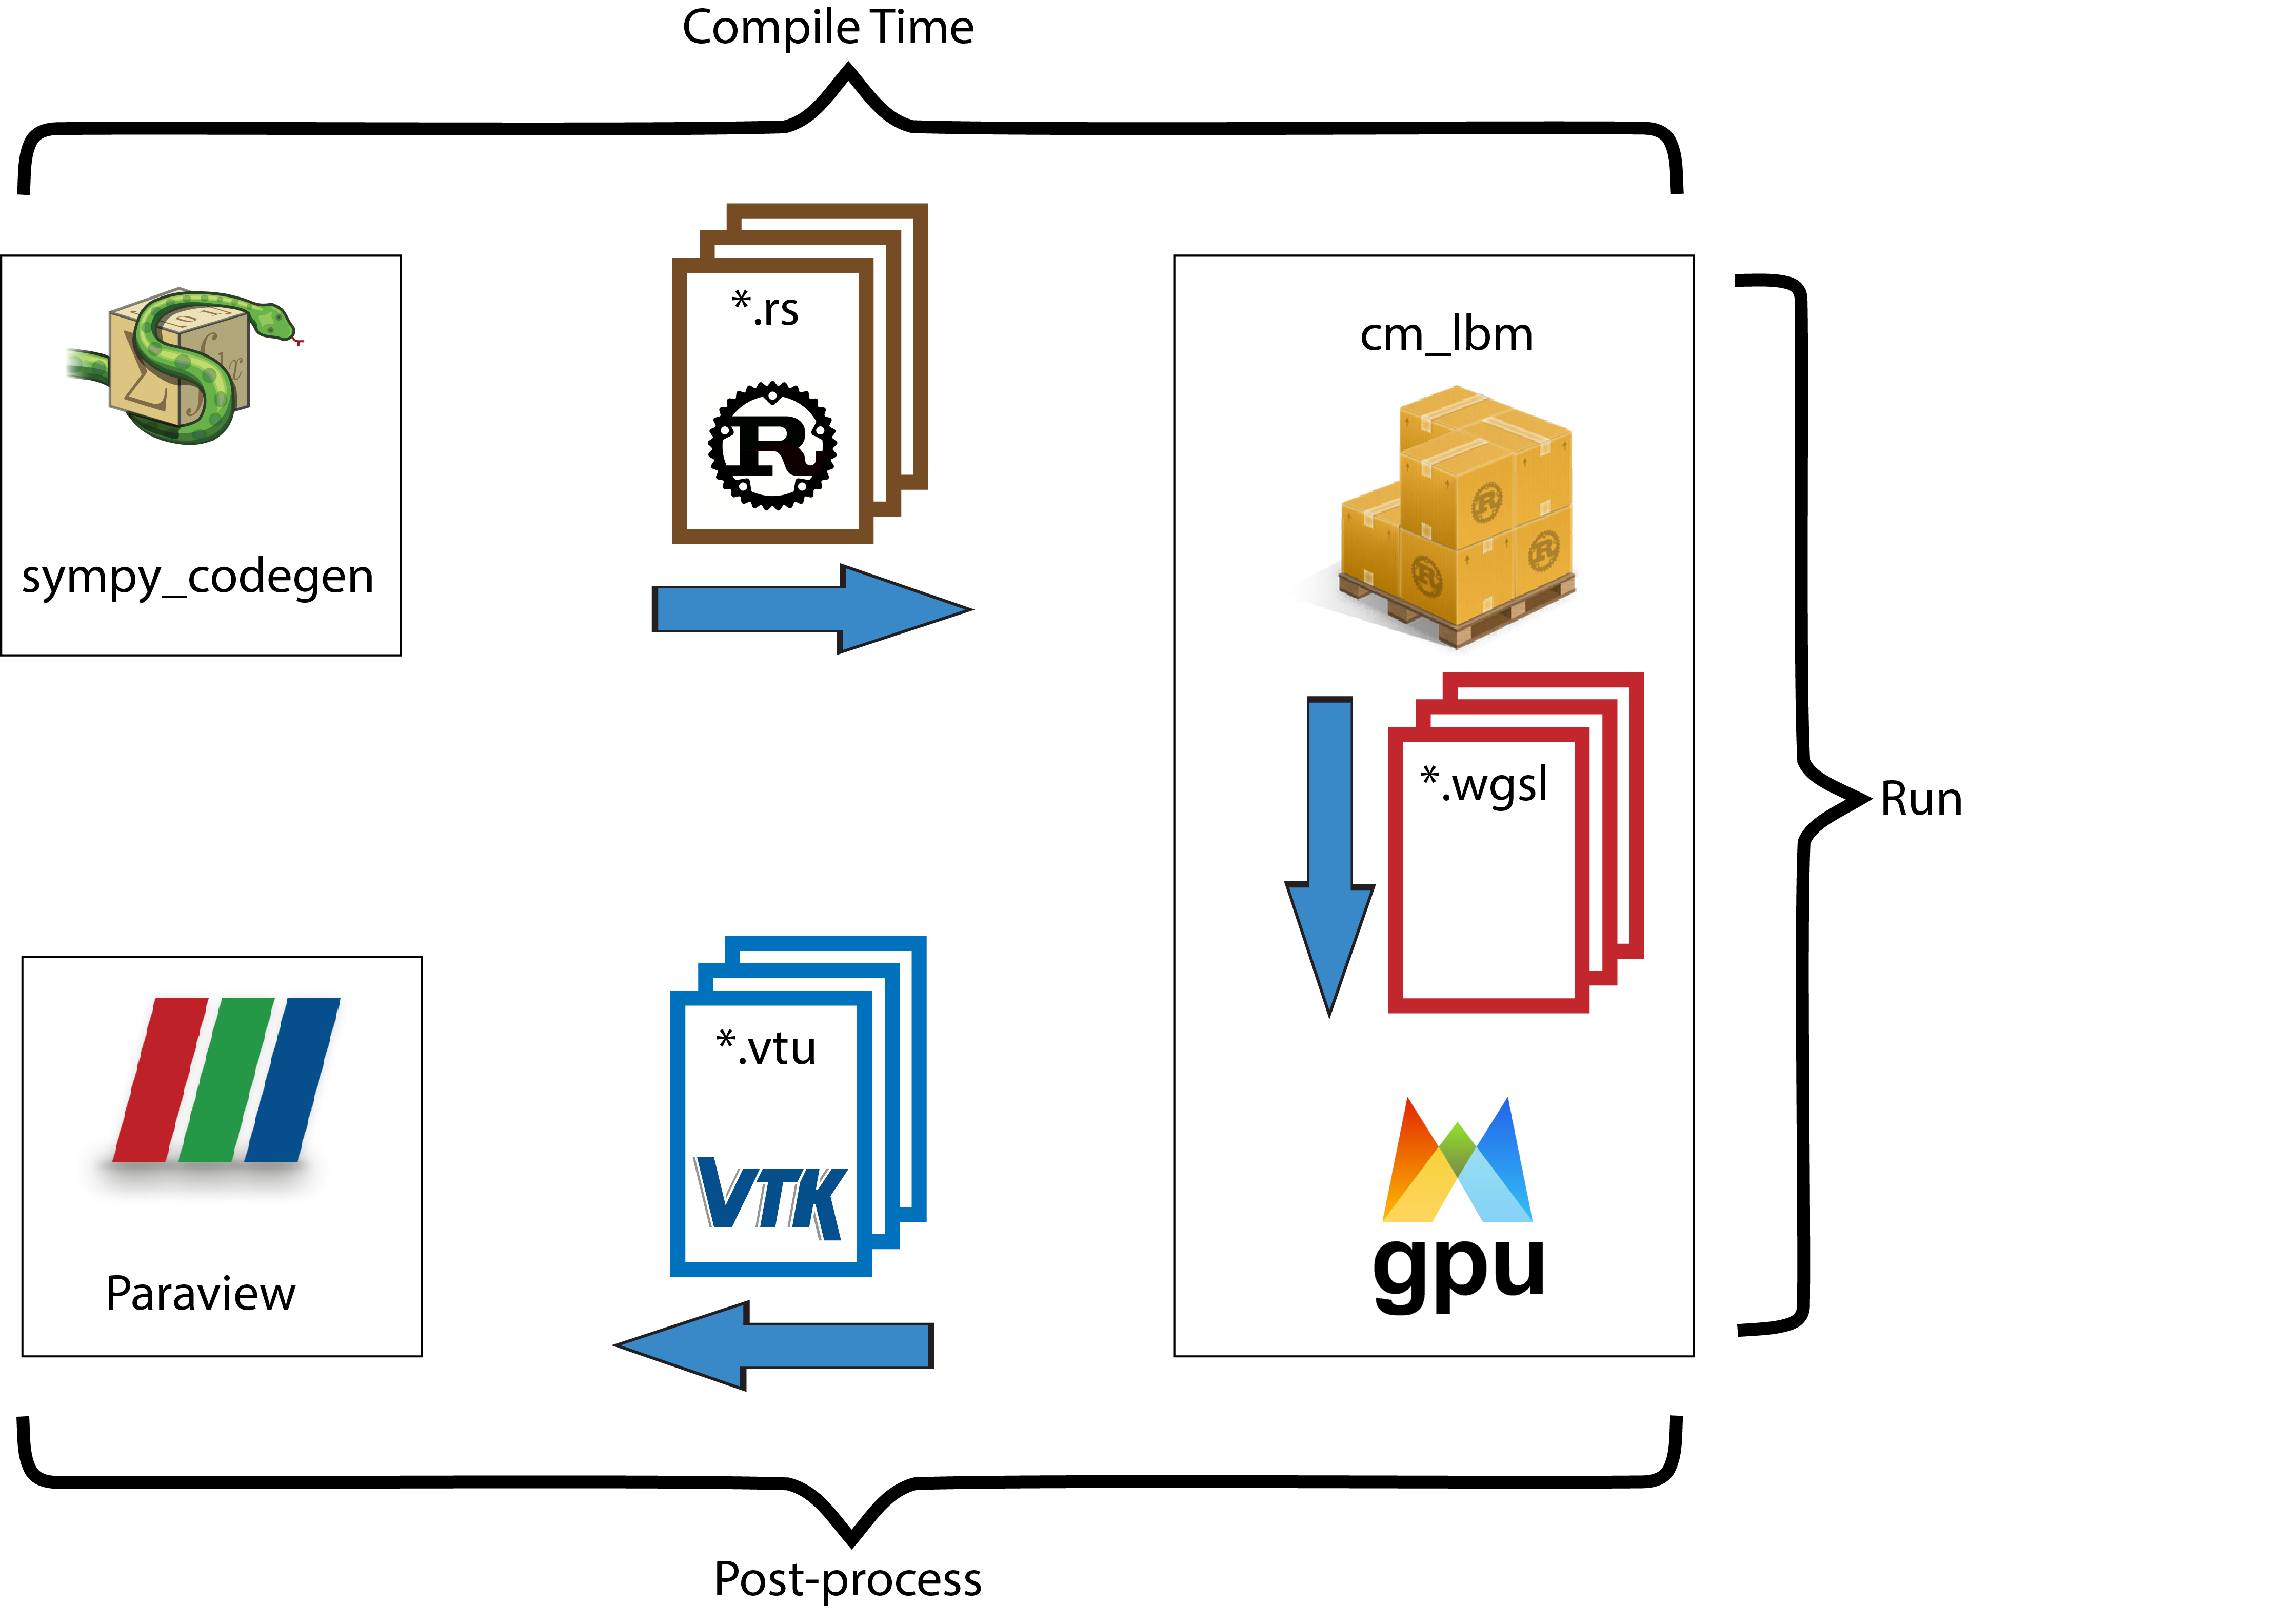
\includegraphics[width=0.8\linewidth]{workflow.png}
\end{center}
  \caption{The architecture of our project has three main components.
  \lstinline{sympy_codegen} generates rust code 
  for the core LBM operators, and is written in Python using SymPy.
  These source files are then compiled into \lstinline{cm_lbm},
  an application written in Rust that at runtime generates and 
  executes compute shaders targeting WGPU.
  Lastly, a given simulation will output VTK files that can be
  visualized with Paraview.
}
  \label{fig:architecture}
\end{figure*}

\begin{figure}
  \begin{center}
    \includegraphics[width=0.6\linewidth]{group_rainbow.png}
  \end{center}
  \caption{The collision operator and applying boundary conditions are mutually exclusive.
  Here we see how different compute passes handle different parts of the domain.
Green ($xz$ faces) and orange ($yz$ faces) are slip boundaries.
Red ($xy$ faces) enforces the Dirichlet boundary conditions.
Blue (internal) gets the collision operator or specular slip boundary 
depending on the cell type.}
\end{figure}

\begin{figure}
  \begin{center}
    \includegraphics[width=0.4\linewidth]{stream_0.png}
    \includegraphics[width=0.4\linewidth]{stream_1.png}

    \includegraphics[width=0.6\linewidth]{stream_2.png}
  \end{center}
  \caption{Stream example}
\end{figure}

\begin{figure}
  \begin{center}
    \includegraphics[width=\linewidth]{specular.png}
  \end{center}
  \caption{Specular Slip Boundaries.
For now we can add spheres, here we see those cells colored by the z component of the normal.}
\end{figure}
